\subsection{String Representation}

With the next SDM, we shall create a string representation for a complete learning box. To accomplish this, we have to iterate through all cards in all
partitions which involves an inner loop nested in an outer loop. SDMs support arbitrary nesting of For Each story nodes via special guards. In
Sec.~\ref{sec:empty} we already used the \texttt{[end]} edge guard to terminate a loop and, as depicted in \note{[each time]}Fig.~\ref{fig:sdm_tostring_1}, an
\texttt{[each time]} guard is used to indicate control flow that is \emph{nested} in the For Each story node and is executed for each match.

Go ahead and create the SDM for \texttt{Box::toString} until it closely resembles Fig.~\ref{fig:sdm_tostring_1}. The first For Each \texttt{ForAllPartitions}
matches all partitions and each partition is used \texttt{[each time]} in \texttt{ForAllCards} to match all cards. Note that \texttt{partition} in
\texttt{ForAllCards} is bound  and thus refers to the assigned value determined in \texttt{ForAllParitions}. When all cards have been matched,
\texttt{ForAllCards} terminates or \texttt{[end]}s and returns to the outer loop \texttt{ForAllPartitions}.

\begin{figure}[htbp]
\begin{center}
  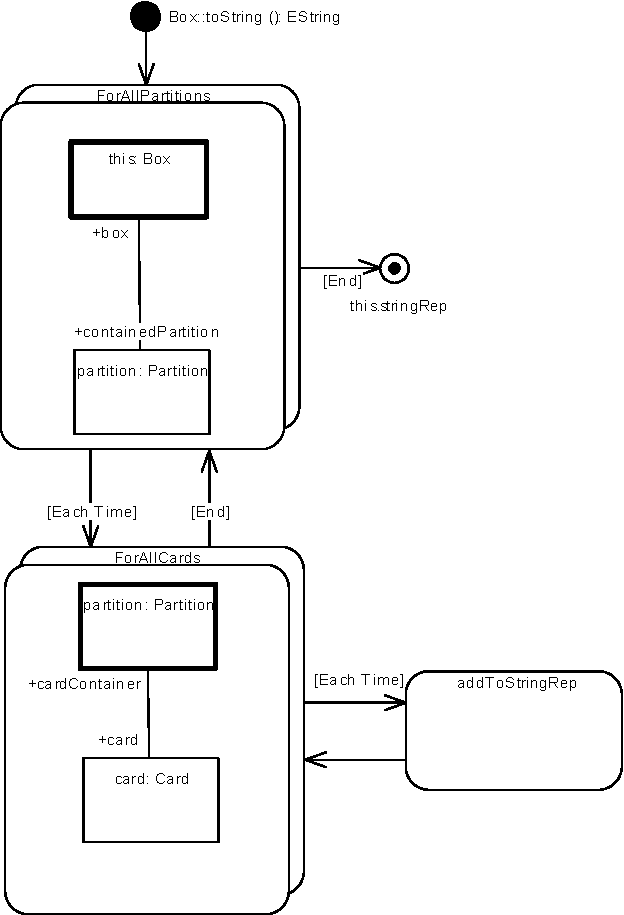
\includegraphics[width=0.8\textwidth]{ea_nestedControl.pdf}
  \caption{Control flow with nested loops.}  
  \label{fig:sdm_tostring_1}
\end{center}
\end{figure}

To actually do something sensible with each card, double-click the empty activity node that is taken each time a card is matched and invoke the \texttt{Edit
ActivityNode} dialogue. Now choose \texttt{addToStringRep} as the name, and \texttt{StatementNode} as the type of the activity node
(Fig.~\ref{fig:sdm_tostring_2}). \note{Statement Nodes} A statement node is used to invoke a method from a class in any package in the current EA project via a
MethodCallExpression. This way, the method invocation is represented as an activity node and is guaranteed to be executed at this point in the control flow.

\begin{figure}[htbp]
\begin{center}
  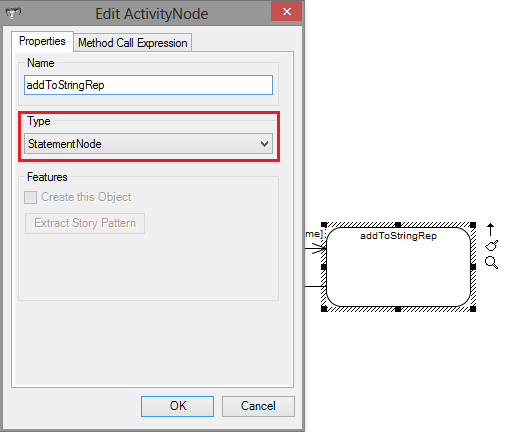
\includegraphics[width=0.8\textwidth]{ea_createStatementNode.png}
  \caption{Invoking a method in a \texttt{StatementNode}.}  
  \label{fig:sdm_tostring_2}
\end{center}
\end{figure}

As we have already used a MethodCallExpression in an attribute constraint (Sec.~\ref{sec:sdm_grow}), go ahead and click the \texttt{Method Call Expression} tab
and select \texttt{MethodCallExpression} as expression, \texttt{this} as target, \texttt{addToStringRep} as operation and \texttt{card} as value of the
parameter (Fig.~\ref{fig:sdm_tostring_3}). That way, we pass the object variable \texttt{card} to the method \texttt{addToStringRep} as parameter.

Statement nodes should be used to interact with methods that are implemented by hand and provide a means of invoking libraries and arbitrary Java code from
SDMs. Please note that we do not differentiate at this point between methods that are implemented via an SDM or by hand and thus, statement nodes can
\note{Recursion} of course be used to invoke other SDMs via a MethodCallExpression. Most importantly, this enables \emph{recursion} as the current SDM can be
invoked on \texttt{this} with appropriate new arguments.

A final point to note is that the return value of the method is ignored -- statement nodes are therefore best used for void methods that either have appropriate
side effects (e.g. manipulate their arguments). We shall learn in a few pages how to invoke methods with non-primitive return values (if a method returns a
primitive then it can be invoked in an attribute constraint as in Sec.~\ref{sec:sdm_grow}).

% \begin{figure}[htbp]
% \begin{center}
%   \includegraphics[width=0.4\textwidth]{pics/sdmBilder/toString/sdm74.png}
%   \caption{Specify a \texttt{MethodCallExpression} in the
%   \texttt{StatementNode}.}
%   \label{fig:sdm_tostring_3}
% \end{center}
% \end{figure}

To complete the SDM, return the final string representation of the box via an \texttt{AttributeValueExpression} in the stop node (Fig.~\ref{fig:sdm_tostring_4}). 


\begin{figure}[ht]
   \centering
      \subfloat[Specify a \texttt{MethodCallExpression} in the \texttt{StatementNode}.]{
        \includegraphics[width=0.4\textwidth]{sdm74}
      }\qquad
      \subfloat[Using a \texttt{AttributeValueExpression} as a return value.]{
        \includegraphics[width=0.45\textwidth]{sdm75}
        \label{fig:sdm_tostring_4}
      }
      \caption{}
\end{figure}
\FloatBarrier

% \begin{figure}[htbp]
% \begin{center}
%   \includegraphics[width=0.5\textwidth]{pics/sdmBilder/toString/sdm75.png}
%   \caption{Using a \texttt{AttributeValueExpression} as a return value.}  
%   \label{fig:sdm_tostring_4}
% \end{center}
% \end{figure}

Take some time to compare and reflect on the complete SDM as depicted in Fig.~\ref{fig:sdm_tostring_5}.  The idea was to abstract from the actual text
representation of the box and model the necessary traversal of the data structure. The helper methods \texttt{addToStringRep}could, for example, build up a
string buffer and update this string representation. While modelling this SDM, we have seen that for each story nodes can be nested, and have learnt two new
uses of MethodCallExpressions that provide a type safe\footnote{Apart from the literal expressions used for specifying argument values.} means of invoking
methods from SDMs.

\begin{figure}[htbp]
\begin{center}
  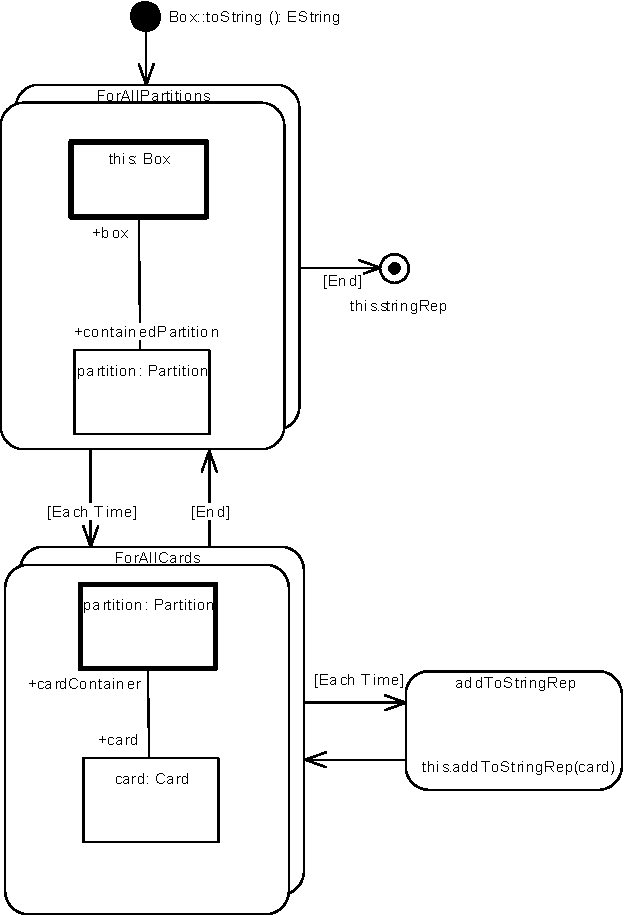
\includegraphics[width=0.75\textwidth]{ea_completeActivityStringRep.pdf}
  \caption{The complete SDM for \texttt{Box::toString}.}  
  \label{fig:sdm_tostring_5}
\end{center}
\end{figure}
\FloatBarrier